In this section, we describe the lattice representation used to model
array values for the analyses in this chapter.
Constant propagation for scalar variables has historically been performed
by efficient dataflow analysis
or
abstract interpretation techniques in which values of variables are
modeled as {\it lattice elements}~\cite{Kild73,WeZa91}.
Given a scalar variable $v$,
the usual approach is to allow
the value of its lattice element
$\L(v)$ to be $\top$, $Constant$ or
$\bot$.  When $\L(v)$ is $Constant$, the lattice
element also contains the value of
the constant\footnote{
An extension that is sometimes employed is to also include
lattice elements that can represent a
small set of constants or a range of constants\cite{Harr77}.
This functionality is not addressed in our chapter, but would be
a straightforward extension to our framework.}.

Formally, a lattice used for scalar constant
propagation consists of:
\begin{enumerate}
\item A set of lattice elements:
a lattice element for a program variable $v$ is written
as $\L(v)$, and denotes $\Set(\L(v))$~=~a set of possible values for
variable $v$.

\item $\top$ (``top'') and $\bot$ (``bottom''), two distinguished
elements of $\L$.
The sets denoted by these lattice elements are
$\Set(\top) = \{\;\}$ (the empty set), and $\Set(\bot) = \U^v$,
where $\U^v$ is the universal set of values for variable
$v$.
\item  If $\L(v)$ is a $Constant$ lattice element
$\Set(\L(v)) = \{Constant\}$, the singleton set containing a constant.
\item A {\it join}
operator, $\sqcap$, such that for any lattice element $e$,
$e \sqcap \top = e$ and $e \sqcap \bot = \bot$. 

The $\sqcap$ operator on lattice elements corresponds to the set {\it union}
operation on the sets denoted by lattice elements
\ie\ if $e$ and $f$ are two lattice elements, then 
$\Set(e \sqcap f) = \Set(e) \cup \Set(f)$.

It follows that the $\sqcap$
operator is idempotent, commutative, and associative, and 
that the lattice is {\it complete} \ie\ $\sqcap$ is closed
on $\L$.
\item A $\sqsupseteq$ operator such that $e \sqsupseteq f$ if and only if
$e \sqcap f = f$, and a $\sqsupset$ operator such that $e \sqsupset f$
if and only if $e \sqsupseteq f$ and $e \not= f$.

The $\sqsupseteq$ and $\sqsupset$ operators on lattice elements
correspond to the {\it inclusive subset} and {\it proper subset}
operations on the sets denoted by lattice elements \ie\
$e \sqsupseteq f$ if and only if $\Set(e) \subseteq \Set(f)$, and
$e \sqsupset f$ if and only if $\Set(e) \subset \Set(f)$.

The $\sqsupset$ operator defines a partial order on lattice elements.
If $e \sqsupset f$, we say that $e$ is ``above'' $f$ and that $f$ is ``below''
$e$ in the lattice.  Hence, $\top$ is above all other lattice elements
and $\bot$ is below all other lattice elements.
\end{enumerate}
The {\it height} $H$ of lattice $\L$ is the length of the largest 
sequence of lattice elements $e_1, e_2, \ldots, e_H$ such that
$e_i \sqsupset e_{i+1}$ for all $1 \leq i < H$. The height of the
lattice for scalar constant propagation is 3.


We now describe how lattice elements for array variables are represented in 
our framework for constant propagation.
Let $\U^A_{ind}$ and $\U^A_{elem}$ be the universal set of {\it index values}
and the universal set of array {\it element values} respectively
for an array variable $A$
in Array SSA form.
For an array variable,
the set denoted by
lattice element $\L(A)$ is a subset of $\U^A_{ind} \times \U^A_{elem}$ \ie\
a set of index-element pairs.
There are three kinds of lattice elements for array variables that are of
interest in our framework:
\begin{enumerate}
\item $\L(A) = \top \;\;\imp\;\; \Set(\L(A)) = \{\;\}$\\
This ``top'' case indicates that the set of possible index-element
pairs
that have been identified thus far for $A$ is the empty set, $\{\;\}$.


\item $\L(A) = \langle(i_1,e_1), (i_2,e_2), \ldots\rangle$\\
$\imp\;\; \Set(\L(A)) = \{ (i_1,e_1), (i_2,e_2), \ldots \} \;\cup\;
(\U^A_{ind}-\{i_1,i_2,\ldots\})\times \U^A_{elem}$\\
In general,
the lattice element for this ``constant'' case is represented by a finite
list
of index-element pairs, $\langle(i_1,e_1), (i_2,e_2), \ldots\rangle$
where $i_1, i_2, \ldots$ are constant index values, and 
$e_1, e_2, \ldots$ are constant element values.
The constant indices, $i_1, i_2, \ldots$, must represent distinct (non-equal)
index values.  As in the scalar case,
the lattice ordering ($\sqsupset$) for these  elements is determined by the subset
relationship among the sets that they denote.


The meaning of this ``constant'' lattice element is
that the current stage of analysis
has identified some finite number of constant index-element pairs
for array variable $A$, such
that $A[i_1] = e_1$, $A[i_2] = e_2$, etc.
All other elements of $A$ are assumed to be non-constant.
(Extensions to handle non-constant indices are
described in section~\ref{sec:non-const}.)

\item $\L(A) = \bot \;\;\imp\;\; \Set(\L(A)) =  \U^A_{ind} \times \U^A_{elem}$\\
This ``bottom''
case indicates that, according to
the approximation in the current stage of analysis, array $A$ may take on any
value from the universal set of index-element pairs.
Note that $\L(A)=\bot$ is equivalent to an empty list,
$\L(A)=\langle \; \rangle$, in case (2) above; they both 
denote the universal set of index-element pairs.
\end{enumerate}

\begin{figure}%[tbp]
\centerline{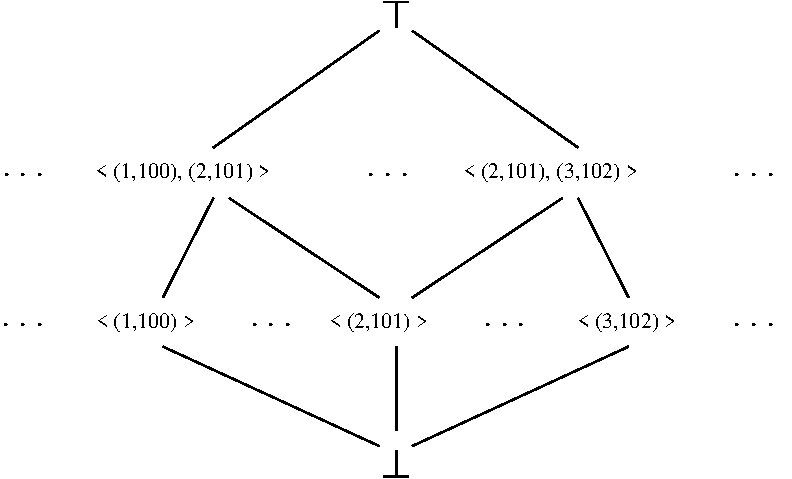
\includegraphics{array2.pdf}}
\caption{Lattice elements of array values with maximum list size \protect{$Z=2$}}
\label{fig:array2}
\end{figure}

Regardless of the size of an array, $A$, the number
of index-element pairs in  $\L(A)$ is bounded by the number of
static assignments to $A$ in the source. 
For the sake of efficiency, we will further restrict the constant array lattice
elements, $\L(A) = \langle(i_1,e_1), (i_2,e_2), \ldots\rangle$,
to lists that are bounded in size by some constant, $Z\geq 1$.
Doing so ensures
that the height of the lattice for array values is at most $(Z+2)$,
which in turn bounds the worst-case complexity of analysis algorithms
that use these lattice elements by a constant factor or at most $(Z+2)$.
If any data flow equation yields a lattice element with $>Z$ pairs, then
this size constraint can be obeyed by conservatively dropping 
index-element pairs
from the list till there are $<= Z$ pairs remaining.  Note that if
lattice element $\L_2$ is obtained by dropping one or more index-element pairs
from lattice element $\L_1$, then it must be the case that 
$\Set(\L_1) \subset \Set(\L_2)$ and that $\L_1  \sqsupset \L_2$ \ie\ 
$\L_2$ is below $\L_1$ in the lattice.  Hence it is always correct (though
conservative) to approximate $\L_1$ by $\L_2$.


If an array assignment statement only modifies a single element, the
lattice element for the real (non-$\phi$) definition in Array SSA form
will contain at most one constant
index-element pair.  However, the lattice
value for the corresponding definition $\phi$ can potentially be
larger in size, since it may carry forward a large number of constant
index-element pairs from previous definitions.  That is why we impose
the size limit of $Z$ on lists of index-element pairs.  The choice of
an appropriate value of $Z$ is an implementation decision depending on the
desired trade-off between precision in program analysis and compile-time
overhead.


\begin{figure}%[tbp]
\centerline{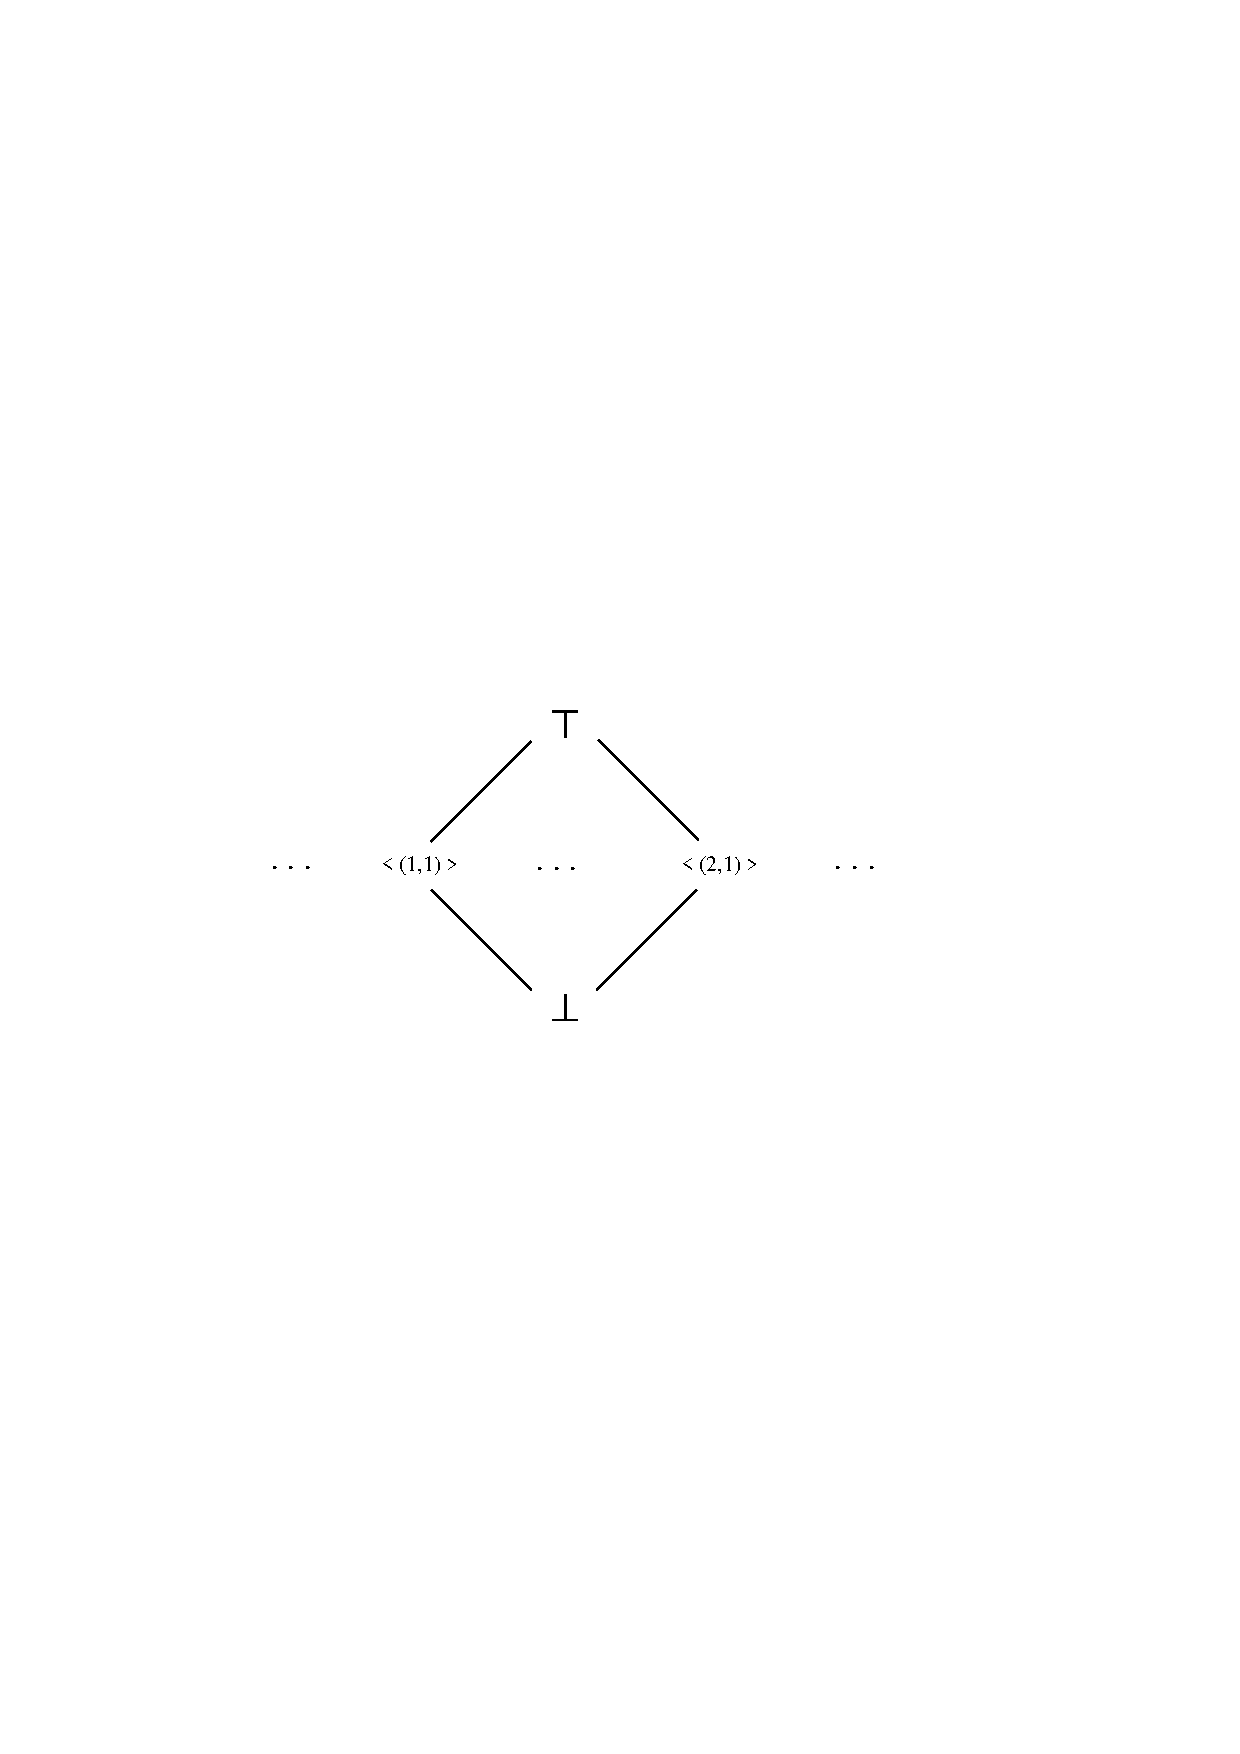
\includegraphics{array1.pdf}}
\caption{Lattice elements of array values with maximum list size \protect{$Z=1$}}
\label{fig:array1}
\end{figure}

\begin{figure}%[tbp]
\centerline{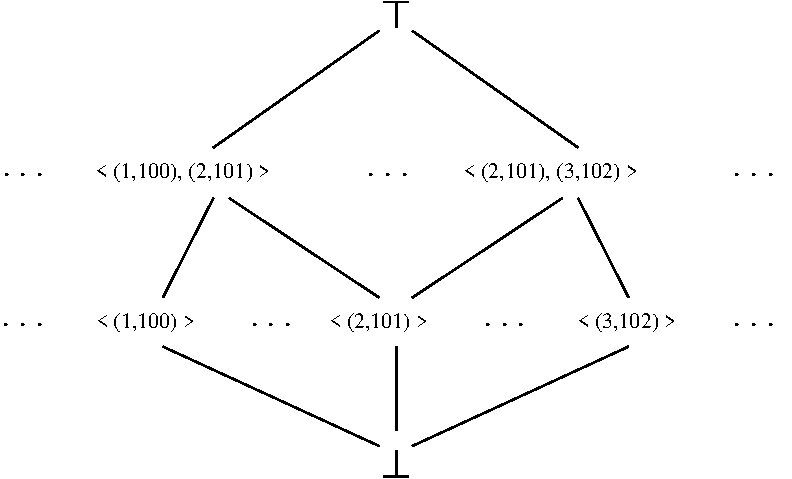
\includegraphics{array2.pdf}}
\caption{Lattice elements of array values with maximum list size \protect{$Z=2$}}
\label{fig:array2}
\end{figure}

The lattice structure for the $Z=1$ case is shown in figure~\ref{fig:array1}.  This lattice has three levels, just like scalar constants.  The middle level contains all possible singleton
ordered lists \ie\ lists  that contain a single constant index-element pair.

The lattice structure for the $Z=2$ case is shown in figure~\ref{fig:array2}.  This lattice has four levels.  The second level (just below $\top$)
contains all possible 
lists that contain exactly two constant index-element pairs.  The third level (just above $\bot$) contains all possible 
lists that contain a single constant index-element pair.  
As mentioned earlier,
the lattice ordering is determined by the subset relationship among the sets denoted by the lattice elements.  For example, consider two lattice elements $\L_1 = \langle(1,100), (2,101)\rangle$ and $\L_2 = \langle(2,101)\rangle$.  The sets denoted by these lattice elements are:
\begin{eqnarray*}
\Set(\L_1) & = & \{(1,100), (2, 101)\} \;\cup\;\;
(\U_{ind} - \{1,2\}) \times \U_{elem} \\
\Set(\L_2) & = & \{(2, 101)\} \;\cup\;\;
(\U_{ind} - \{2\}) \times \U_{elem}
\end{eqnarray*}
Therefore, $\Set(\L_1)$ is a proper subset of $\Set(\L_2)$ and we have $\L_1 \sqsupset \L_2$ \ie\ $\L_1$ is above $\L_2$ in the lattice in figure~\ref{fig:array2}.


\begin{figure}%[htbp]
\begin{center}
\begin{tabular}{|l||c|c|c|}
\hline
$\L(A_1[k])$ & $\L(k) = \top$ & $\L(k) = Constant$ & $\L(k) = \bot$ \\
\hline \hline
$\L(A_1) = \top$ & $\top$ & $\top$ & $\bot$ \\
\hline
$\L(A_1) = \langle (i_1,e_1), \ldots \rangle$ & $\top$ & $e_j$, 
if $\exists$
$(i_j,e_j) \in \L(A_1)$ with &\\
& & $\DS(i_j, \L(k)) = \mbox{\it true}$ & $\bot$\\
& & $\bot$, otherwise & \\
\hline
$\L(A_1) = \bot$ & $\bot$ & $\bot$ & $\bot$ \\
\hline
\end{tabular}
\end{center}
\caption{Lattice computation for \protect{$\L(A_1[k]) = \L_{[\:]}(\L(A_1), \L(k))$},
where $A_1[k]$ is an 
array element read operator}
\label{fig:aref}
\end{figure}

\begin{figure}%[htbp]
\begin{center}
\begin{tabular}{|l||c|c|c|}
\hline
$\L(A_1)$ & $\L(i) = \top$ & $\L(i) = Constant$ & $\L(i) = \bot$ \\
\hline \hline
$\L(k) = \top$ & $\top$ & $\top$ & $\bot$ \\
\hline
$\L(k) = Constant$ & $\top$ & $\langle(\L(k),\L(i))\rangle$ & $\bot$ \\
\hline
$\L(k) = \bot$ & $\bot$ & $\bot$ & $\bot$ \\
\hline
\end{tabular}
\end{center}
\caption{Lattice computation for \protect{$\L(A_1) = \L_{d[\:]}(\L(k), \L(i))$},
where $A_1[k] := i$ is an 
array element write operator}
\label{fig:adef}
\end{figure}

We now describe how array lattice elements are computed for various
operations that appear in Array SSA form.  We start with the simplest operation
\viz\ a reference (read access) to an array element.
Figure~\ref{fig:aref} shows how $\L(A_1[k])$, the lattice element for array
reference $A_1[k]$, is computed as a function of $\L(A_1)$ and $\L(k)$, 
the lattice elements for $A_1$ and $k$.
We denote this function
by $\L_{[\:]}$ \ie\ $\L(A_1[k]) = \L_{[\:]}(\L(A_1),\L(k))$.  
The interesting case in figure~\ref{fig:aref} occurs
in the middle cell
when neither $\L(A_1)$ nor $\L(k)$ is $\top$ or $\bot$.
In this case, $\L(k) = Constant$ and $\L(A_1)$ is a nonempty list of the form,
$\langle (i_1,e_1), \ldots \rangle$.  For this case, if there exists
an index-element
pair $(i_j, e_j)$ in $\L(A_1)$ such that $i_j$ is the same as the constant
$\L(k)$, then the value returned for $\L(A_1[k])$ is the constant $e_j$.
Otherwise, $\bot$ is returned as the value for $\L(A_1[k])$.

The notation $\DS$ in the middle cell in figure~\ref{fig:aref}
represents a ``definitely-same'' binary relation \ie\ $\DS(a,b) =
\mbox{\it true}$ if and only if $a$ and $b$ are known to have exactly
the same value.  If, as in the current discussion, $a$ and $b$ are
constants then $\DS(a,b) = \mbox{\it true}$ if and only if $a=b$.
However, we use the $\DS$ notation for generality because later in
section~\ref{sec:non-const} we show how the lattice modeling of arrays
introduced in this section can be extended to symbolic index values.

Next, consider a definition (write access) of an array element, which 
in general has the form $A_1[k] := i$.
Figure~\ref{fig:adef} shows how $\L(A_1)$, the lattice element for 
the array being written into,
is computed as a function of $\L(k)$ and $\L(i)$, 
the lattice elements for $k$ and $i$.  We denote this function
by $\L_{d[\:]}$ \ie\ $\L(A_1) = \L_{d[\:]}(\L(k),\L(i))$.  
As before,
the interesting case in figure~\ref{fig:adef} occurs
in the middle cell
when both $\L(k)$ and $\L(i)$ are constant.
For this case, the value returned for $\L(A_1)$ is simply 
the singleton list,
$\langle\;(\L(k),\L(i))\;\rangle$, which contains exactly
one constant index-element pair.


Now, we turn our attention to the $\phi$ functions. 
Consider a
definition $\phi$ operation
of the form, $A_2 := d\phi(A_1, A_0)$.  
The lattice computation for $\L(A_2) = \L_{d\phi}(\L(A_1), \L(A_0))$
is shown in figure~\ref{fig:dphi}.  Since $A_1$ corresponds to a definition
of a single array element, the list for $\L(A_1)$ can contain
at most one pair (see figure~\ref{fig:adef}).
Therefore, the three cases considered for $\L(A_1)$ in figure~\ref{fig:dphi}
are $\L(A_1) = \top$, $\L(A_1) = \langle(i',e')\rangle$, and
 $\L(A_1) = \bot$.

The notation 
$\Update((i',e'),\langle (i_1,e_1), \ldots \rangle)$
used in the middle cell in 
figure~\ref{fig:dphi} denotes a special update of 
the list $\L(A_0) = \langle (i_1,e_1), \ldots \rangle$
with respect to the constant
index-element pair $(i',e')$. $\Update$ involves four steps\label{def:update}:
\begin{enumerate}
\item Compute the list $T = \{\;(i_j,e_j)\;|\;(i_j,e_j)\in\L(A_0)
\mbox{~and~}\DD(i',i_j)=\mbox{\it true}\;\}$.  List $T$
contains only those pairs from $\L(A_0)$ that have an index
value $i_j$ that is {\it definitely different} from $i'$.

Analogous to $\DS$, $\DD$ denotes a ``definitely-different'' binary
relation \ie $\DS(a,b) = \mbox{\it true}$ if and only if $a$ and
$b$ are known to have distinct (non-equal) values.

\item Insert the pair $(i',e')$ into $T$ to obtain a new list, $I$.
\item If the 
size of list
$I$ exceeds the threshold size $Z$, then one of the pairs in $I$ is
dropped from the output list so as to satisfy the size constraint.  
(Since the size of $\L(A_0)$ must have been $\leq Z$, it is sufficient
to drop only one pair to satisfy the size constraint.)
\item Return $I$ as the value of 
$\Update((i',e'),\langle (i_1,e_1)\
, \ldots \rangle)$.
\end{enumerate}

\begin{figure}%[htbp]
\begin{center}
\begin{tabular}{|l||c|c|c|}
\hline
$\L(A_2)$ & $\L(A_0) = \top$ & $\L(A_0) = \langle (i_1,e_1), \ldots \rangle $ & $\L(A_0) = \bot$ \\
\hline \hline
$\L(A_1) = \top$ & $\top$ & $\top$ & $\top$ \\
\hline
$\L(A_1) = \langle(i',e')\rangle$ & $\top$ & $\Update((i',e'),\langle (i_1,e_1), \ldots \rangle)$ & $\langle(i',e')\rangle$ \\
\hline
$\L(A_1) = \bot$ & $\bot$ & $\bot$ & $\bot$ \\
\hline
\end{tabular}
\end{center}
\caption{Lattice computation for \protect{$\L(A_2)  =  \L_{d\phi}(\L(A_1), \L(A_0))$}
where $A_2 := d\phi(A_1, A_0)$ is
a definition $\phi$ operation}
\label{fig:dphi}
\end{figure}


\begin{figure}%[htbp]
\begin{center}
\begin{tabular}{|l||c|c|c|}
\hline
$\L(A_2) = \L(A_1) \sqcap \L(A_0) $ & $\L(A_0) = \top$ & $\L(A_0) = \langle (i_1,e_1), \ldots \rangle $ & $\L(A_0) = \bot$ \\
\hline \hline
$\L(A_1) = \top$ & $\top$ & $\L(A_0)$ & $\bot$ \\
\hline
$\L(A_1) = \langle(i'_1,e'_1), \ldots\rangle$ & $\L(A_1)$ & $\L(A_1) \cap \L(A_0)$ & $\bot$ \\
\hline
$\L(A_1) = \bot$ & $\bot$ & $\bot$ & $\bot$ \\
\hline
\end{tabular}
\end{center}
\caption{Lattice computation for 
$\L(A_2) = \L_{\phi}(\L(A_1), \L(A_0)) = \L(A_1) \sqcap \L(A_0) $,
where $A_2 := \phi(A_1, A_0)$ is
a control $\phi$ operation}
\label{fig:join}
\end{figure}

Finally,
consider a control $\phi$ operation that merges two array values, $A_2 := \phi(A_1, A_0)$.
The join operator ($\sqcap$) is used to compute $\L(A_2)$,
the lattice element for $A_2$, as a function of 
$\L(A_1)$ and $\L(A_0)$,
the lattice elements for $A_1$ and $A_0$ 
\ie\ $\L(A_2) = \L_{\phi}(\L(A_1), \L(A_0)) = \L(A_1) \sqcap \L(A_0)$.
The rules for computing this
join operator are shown in figure~\ref{fig:join}, depending on
different cases for $\L(A_1)$ and $\L(A_0)$.
The notation $\L(A_1) \cap \L(A_0)$ used in the middle cell in
figure~\ref{fig:join} denotes a simple intersection of lists $\L(A_1)$ and 
$\L(A_0)$  --- the result is a list of pairs that appear in both
$\L(A_1)$ and 
$\L(A_0)$.


We conclude this section by discussing the
example program in figure~\ref{fig:sc-ex-source}.  The
partial Array SSA form for this example is shown in
figure~\ref{fig:sc-ex-ssa}, and 
the data
flow equations for this example are shown in
figure~\ref{fig:sc-ex-df}. Each assignment statement
in the partial Array SSA form
(in figure~\ref{fig:sc-ex-ssa})
results in one data flow equation
(in figure~\ref{fig:sc-ex-df}); the numbering S1 through S8
indicates the correspondence.
In general, each data flow equation in our framework has a
single lattice variable on its LHS (Left Hand Side).  Also, a lattice
variable will only appear on the LHS of at most one equation.

The lattice operations ($\L_{\phi}$, $\L_{d\phi}$,  $\L_{[\ ]}$, $\L_{d[\ ]}$,
$\L_*$)
in figure~\ref{fig:sc-ex-df}
depend on the
operations within the corresponding
statements. For example, there are
reads of array elements in the RHS of statements S3 and S5, writes of 
array elements in the LHS of statements S3 and S5, 
definition $\phi$ operators in statements S4 and S6, and a control
$\phi$ operator in statement S7.
We also incorporate lattice computations 
for specific
arithmetic operators such as lattice function $L_*$ for
the multiply operator
in statements S3 and S5. Tables for
lattice computations such as $L_*$ 
are straightforward and are not shown. 
%Operation specific lattice
%computations are used in scalar constant propagation as well.


\begin{figure}%[htbp]

\begin{center}
\parbox{3.0in}{
\begin{programa}
\Ta $Y[3] := 99$ \\
\Ta if $C$ then \\
\Tb   $D[1] := Y[3] * 2$ \\
\Ta else \\
\Tb   $D[1] := Y[I] * 2$ \\
\Ta endif \\
\Ta $Z := D[1]$ 
\end{programa}
}
\end{center}
\caption{Sparse Constant Propagation Example}
\label{fig:sc-ex-source}
\end{figure}

\begin{figure}%[htbp]
\begin{center}
\parbox{3.0in}{
\begin{programa}
\Tb $Y_0$ and $D_0$ in effect here. \\
\Tb  ... \\
\mbox{S1:}\Tb \parbox{1.5in} {$Y_1[3] := 99$}  \\
\mbox{S2:}\Tb \parbox{1.5in} {$Y_2 := d\phi(Y_1,Y_0)$}  \\
\Tb  if $C$ then \\
\mbox{S3:}\Tb \parbox{1.5in} {$\ \ D_1[1] := Y_2[3] * 2$}  \\
\mbox{S4:}\Tb \parbox{1.5in} {$\ \ D_2 := d\phi(D_1,D_0)$}  \\
\Tb else \\
\mbox{S5:}\Tb \parbox{1.5in} {$\ \ D_3[1] := Y_2[I] * 2$}  \\
\mbox{S6:}\Tb \parbox{1.5in} {$\ \ D_4 := d\phi(D_3,D_0)$}  \\
\Tb endif \\
\mbox{S7:}\Tb \parbox{1.5in} {$D_5 := \phi(D_2,D_4)$}  \\
\mbox{S8:}\Tb \parbox{1.5in} {$Z := D_5[1]$}  \\
\end{programa}
}
\end{center}
\caption{Array SSA form for the Sparse Constant Propagation Example}
\label{fig:sc-ex-ssa}
\end{figure}

\begin{figure}%[htbp]
\begin{center}
\begin{tabular}{r r c l}
\mbox{S1:} & $\L(Y_1)$ & = & $<(3,99)>$ \\
\mbox{S2:} & $\L(Y_2)$ & = & $\L_{d\phi} (\L(Y_1), \L(Y_0))$ \\
\mbox{S3:} & $\L(D_1)$ & = & $\L_{d[\ ]}(\L_*(\L_{[\ ]}(\L(Y_2),3)), 2))$ \\
\mbox{S4:} & $\L(D_2)$ & = & $\L_{d\phi} (\L(D_1), \L(D_0))$ \\
\mbox{S5:} & $\L(D_3)$ & = & $\L_{d[\ ]}(\L_*(
\L_{[\ ]}(\L(Y_2),\L(I)))
, 2))$ \\
\mbox{S6:} & $\L(D_4)$ & = & $\L_{d\phi} (\L(D_3), \L(D_0))$ \\
\mbox{S7:} & $\L(D_5)$ & = & $\L_{\phi}(\L(D_2),\L(D_4))$ \\
\mbox{S8:} & $\L(Z)$ & =  & $\L_{[\ ]}(\L(D_5), 1)$
\end{tabular}
\end{center}
\caption{Data Flow Equations for the Sparse Constant Propagation Example}
\label{fig:sc-ex-df}
\end{figure}


